\section{Introduction}
\label{sec:introduction}
% state the learning objective

\par The objective of this laboratory assignment is to study a circuit containing independent and 
linearly dependent voltage and current sources. The circuit also contains 7 resistors, totaling 11 components.\par
The circuit has 8 nodes and 4 meshes. The nodes of the circuit were numbered arbitrarily (from {\it$V_{0}$}  to {\it$V_{7}$} ), and it was considered that {\it node 0} was the ground node. The voltage-controlled current source {\it $I_b$} has a linear dependence on Voltage {\it $V_b$}, of constant {\it $K_b$}. The voltage {\it $V_b$} is the voltage drop at the ends of resistor {\it $R_3$}. The current-controlled voltage source {\it $V_c$} has a linear dependece on current {\it $I_c$}, of constant {\it $K_c$}. The control current {\it $I_c$} is the current that passes through the resistor {\it $R_6$}.
The circuit can be seen in \textbf{Figure~\ref{fig:circuit_t1}}.\par
The values for the resistors, the independent sources and the  constants for the dependent 
sources are presented in \textbf{Table~\ref{tab:python_values}}. These values were obtained using the
Python script provided by the Professor responsable for the laboratory assigment
and using the number 95815 as the seed.\par

In Section~\ref{sec:analysis}, a theoretical analysis of the circuit is
presented using two methods: the mesh analysis and the nodal analysis. In Section~\ref{sec:simulation}, the circuit is analysed by
simulation using the program Ngspice, and the results are compared to the theoretical results obtained in
Section~\ref{sec:analysis}. The conclusions of this study are outlined in
Section~\ref{sec:conclusion}.

\begin{figure}[h] \centering
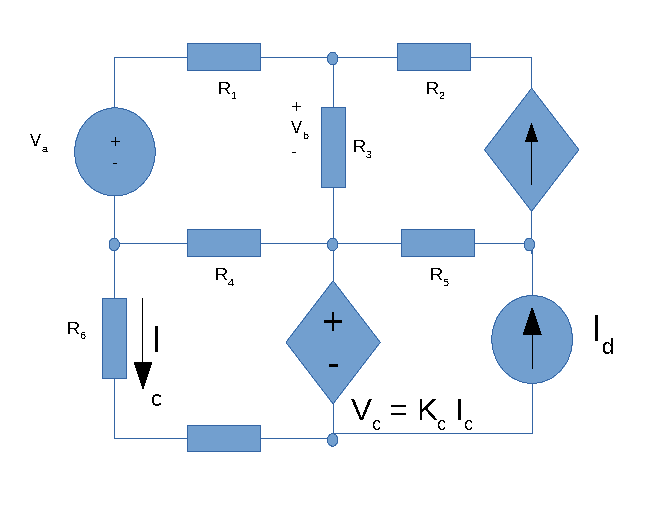
\includegraphics[width=0.9\linewidth]{circuit_t1.pdf}
\caption{Circuit in study}
\label{fig:circuit_t1}
\end{figure}


\begin{table}[h]
  \centering
  \begin{tabular}{|l|r|}
    \hline    
    {\bf Name} & {\bf Python-generated values} \\ \hline
	R1 &  1.04606282456 \\ \hline
	R2 &  2.00732621328 \\ \hline
	R3 &  3.06060705885 \\ \hline
	R4 &  4.07055531265 \\ \hline
	R5 &  3.1225213804 \\ \hline
	R6 &  2.06927045958 \\ \hline
	R7 &  1.01531018068 \\ \hline
	Va &  5.24359648479 \\ \hline
	Id &  1.01891541651 \\ \hline
	Kb &  7.0473187437 \\ \hline
	Kc &  8.3479788681 \\ \hline
	\hline

  \end{tabular}
  \caption{The variables that start with an {\it R} are the values of the resistors 
    and are expressed in  kiloohm  (kOhm); the variable {\it Va} is a {\it voltage} and is expressed in
    Volt (V) and the variable {\it Id}  is a {\it current} and expressed in
   miliAmpere (mA). The constants {\it Kc} and {\it Kb} are  expressed in
   kiloOhm  (kOhm) and miliSiemens (mS), respectively.}
  \label{tab:python_values}
\end{table}

\pagebreak


